% !TeX root = ExtendedAbstract.tex

\section{Background}

\subsection{Persistence Homology}

Persistence homology is a tool developed around 1992 for the purpose of data science. Data scientists had the need to compute the homology of a shape given a finite collection of data points $X$, which raises the question of finding a shape which adequately describes the data. A primitive algorithm consists of picking a positive number $r$ and replacing each data point by a sphere of radius $r$. The resulting open set, denoted $X^{(r)}$, may be understood as an approximation of the real shape underlying the data $X$, and there are efficient algorithms to compute its homology.

\begin{figure}
\centering
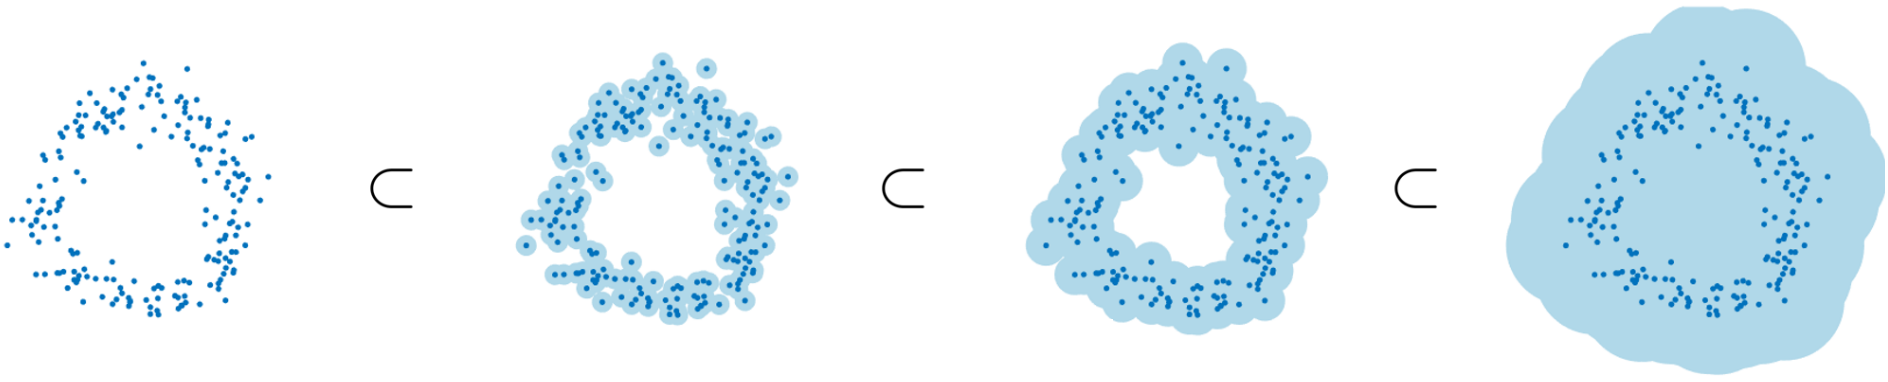
\includegraphics[width=\linewidth]{data}
\caption{Illustration of the sets $X^{(r)}$, with increasing $r$. Note that the middle radii are the ones which better represent the topology of the data. Figure taken from \cite{historypersistence}.}
\end{figure}

This raises the question of which radius $r$ to pick, which requires careful analysis of the data: too small $r$ and the datapoints will be disconnected, too large $r$ and the dataset degenerates into a large ball. However, persistence homology offers an alternative: consider all positive radii at once.

For $k \in \Z$ and $r > 0$, define $H_k^r(X) = H_k(X^{(r)})$, and for $r \leq 0$ set $H_k^r(X) = 0$. These spaces allow us to visualize how the shape of $X^{(r)}$ changes as $r$ increases. Moreover, for $r < s$ the inclusion $X^{(r)} \subseteq X^{(s)}$ induces a natural map $H_k^r(X) \to H_k^s(X)$. This data forms an object which is called a \emph{persistence module}. In the sequence we will be working exclusively with vector spaces, so we assume that the homology is taken with coefficients over a field $\FF$.

\begin{definition}
A persistence module is a family of vector spaces $\{V_t\}_{t \in \R}$ (over a field $\FF$), together with maps $\pi_{st} \colon V_s \to V_t$ for $s \leq t$, such that
\begin{align}
\pi_{tt} &= \id,\\
\pi_{tr} \circ \pi_{st} &= \pi_{sr}, \quad s \leq t \leq r.
\end{align}

Moreover, a persistence module $(\{V_t\}_{t \in \R}, \{\pi_{st}\}_{s\leq t})$ is said to be of \emph{finite type} if the following three conditions are satisfied:
\begin{enumerate}
\item For all but finitely many $t$ there exists a neighborhood $U$ of $t$ such that $\pi_{st}$ is an isomorphism for $s, t \in U$,
\item For all $t \in \R$ there exists $\varepsilon$ such that $\pi_{(t-\delta), t}$ is an isomorphism for all $0 \leq \delta < \varepsilon$,
\item\label{pm3} For all $t \in \R$ close enough to $-\infty$, $V_t = 0$.
\end{enumerate}
\end{definition}

In practice, all the constructions for persistence modules that will be discussed in this thesis originate persistence modules of finite type. This is useful because of an important representation theorem for this class of persistence modules.

\begin{definition}
A \emph{barcode} is a finite multiset\footnote{A multiset is a set whose elements are counted with multiplicity.} of intervals of type $\linterval a b$, with $-\infty < a < b \leq +\infty$. We work under the convention that $\linterval a \infty = \ointerval a \infty$.
\end{definition}

\begin{definition}
Let $B = \{I_1, \dots, I_n\}$ be a barcode. Define the persistence module $\FF(B) = (\{V_t\}_{t \in \R}, \{\pi_{st}\}_{s \leq t})$ as follows
\begin{itemize}
\item Define $V_t = \braket{\,i \mid t \in I_i\,}$, where the brackets denote the free vector space over $\FF$,
\item For $s \leq t$, define $\pi_{st} \colon V_s \to V_t$ by defining it on the basis elements of $V_s$. For every $i$ such that $s \in I_i$,
\begin{itemize}
\item If $t \in I_i$, set $\pi_{st}(i) = i$,
\item Otherwise, set $\pi_{st}(i) = 0$.
\end{itemize}
\end{itemize}

It is straight-forward to prove that $\FF(B)$ is a persistence module of finite type.
\end{definition}

\begin{theorem}[Normal Form Theorem]
Every persistence module of finite type is isomorphic to $\FF(B)$ for exactly one barcode $B$.
\end{theorem}

The normal form theorem is the persistence analogous to the classical theorem in linear algebra that says that every vector space of finite dimension is isomorphic to $\R^n$ for some unique $n$. By property \ref{pm3} of finite type persistence modules, every persistence module `starts out' as the zero vector space, and at some instant in time it `grows a new basis element'. This marks the start of a bar in its barcode. Similarly, whenever the vector space $V_t$ loses a dimension, that is marked by the end of a bar. In this sense, the barcode of a persistence module is an indicator of when dimensions are appearing and disappearing; when applied to the homology of a topological space, \emph{the bars mark the appearance and disappearance of holes in the space as the parameter varies}.

\medskip

Another example, this one of a more geometrical nature, consists of considering a topological space equipped with a sufficient regular fibration, such as one induced by a Morse function. More concretely, let $X$ be a compact manifold and $f \colon X \to \R$ a Morse function on $X$. Define $X_t$, for $t \in \R$, as
\begin{equation}
X_t = \{\, x \in X \mid f(x) < t \,\}.
\end{equation}

Then, for $k \in \Z$ we may define a persistence module by
\begin{equation}
V_t = H_k(X_t),
\end{equation}
with the maps $\pi_{st} \colon V_s \to V_t$ being induced by the inclusion $X_s \hookrightarrow X_t$.

Elementary properties of Morse functions will show that the resulting persistence module is of finite type, and therefore has an associated barcode; this barcode is referred to as \emph{the barcode of $f$} (of dimension $k$).

As a concrete example, let $X$ be the torus, embedded vertically in $\R^3$ as in figure \ref{fig:torus1}. We will calculate the barcode (in dimension $1$) of the height function, whose critical values are $z_1 < z_2 < z_3 < z_4$.
\begin{figure}
\centering
\begin{tikzpicture}
\draw[->] (-2,-3) -- (-2,3.5) node[right] {$z$};

\draw (0,0) ellipse (1.5 and 2.7);
  \begin{scope}
    \clip (1.4,0) ellipse (1.8 and 3);
    \draw[name path global=p1] (-1,0) ellipse (1.2 and 2);
  \end{scope}
  \begin{scope}
    \clip (-1,0) ellipse (1.2 and 2);
    \draw[name path global=p2] (1,0) ellipse (1.2 and 2);
  \end{scope}
  
  
\draw[dashed] (0, 2.7) -- (-1.9, 2.7);
\draw (-1.9,2.7) -- (-2.1,2.7) node[left] {$z_4$};

\draw[dashed] (0, -2.7) -- (-1.9, -2.7);
\draw (-1.9,-2.7) -- (-2.1,-2.7) node[left] {$z_1$};

\node (origin) at (0,0) {};
\node (tr) at (-1.9,0) {};
\node (tl) at (-2.1,0) {};


\path [name intersections={of=p1 and p2}];


\draw[dashed] (origin |- intersection-1) -- (tr |- intersection-1);
\draw (tr |- intersection-1) -- (tl |- intersection-1) node[left] {$z_3$};

\draw[dashed] (origin |- intersection-2) -- (tr |- intersection-2);
\draw (tr |- intersection-2) -- (tl |- intersection-2) node[left] {$z_2$};


\end{tikzpicture}
\caption{An embedding of a torus in $\R^3$}\label{fig:torus1}
\end{figure}

Then, the filtration $X_t$ has the following behavior:
\begin{itemize}
\item For $t \leq z_1$, $X_t = \emptyset$, whose first homology is null;
\item For $z_1 < t \leq z_2$, $X_t$ is a disk, whose first homology is null;
\item For $z_2 < t \leq z_3$, $X_t$ is homeomorphic to a cylinder, and therefore its first homology is $\FF$,
\item At $t = z_3$, a handle is closed, and therefore for $z_3 < t \leq z_4$, $X_t$ has first homology equal to $\FF^2$,
\item Finally, for $t > z_4$ we obtain the full torus, whose first homology is $\FF^2$.
\end{itemize}

The induced maps $\pi_{st}$ can also be computed without much difficulty: they are the inclusions $\FF^n \hookrightarrow \FF^m$.

Now, the value of barcodes makes itself clear, as it allows for a much shorter description of the persistence module above described. The barcode associated to the height function in dimension $1$ is as follows:
\begin{figure}[H]
\centering
\begin{tikzpicture}[xscale=3]
\draw[->,thick] (-0.300,0.000)--(3.300,0.000);
\draw[] (0.000,-0.200)--(0.000,0.200) node[above] {$z_1$};
\draw[] (1.000,-0.200)--(1.000,0.200) node[above] {$z_2$};
\draw[] (2.000,-0.200)--(2.000,0.200) node[above] {$z_3$};
\draw[] (3.000,-0.200)--(3.000,0.200) node[above] {$z_4$};
\draw[(-,thick] (1.000,-0.500)--(3.255,-0.500) node[right] {};
\draw[(-,thick] (2.000,-0.800)--(3.255,-0.800) node[right] {};
\end{tikzpicture}
\caption{Visual representation of the barcode associated to the first homology of the torus in \ref{fig:torus1}.}\label{fig:bctorus}
\end{figure}

\subsection{Filtered Floer Homology}
\label{sec:ph}

Floer homology was developed by Andreas Floer in 1988 in order to attack the so-called Arnol'd conjecture, an important problem in symplectic geometry. Filtered Floer homology consists of an $\R$-graded version of Floer homology, which is suitable for application of persistence homology.

Floer homology can be seen as an analogue of Morse homology happening in contractible loop space, so the reader who is already familiar with Morse theory will want to read the following with that in mind.

Let $(M,\omega)$ be a compact aspherical\footnote{This technical restriction means that any map from the sphere $S^2$ to $M$ is contractible.} symplectic manifold. Define $\LL M$ as the space of contractible smooth loops in $M$, i.e. smooth maps $S^1 \to M$. In order to investigate the number of periodic orbits of a given (possibly time-dependent but periodic) Hamiltonian $H \colon S^1 \times M \to \R$, the so-called \emph{action functional} is introduced:
\begin{equation}
\begin{aligned}
\AA \colon \LL M &\longrightarrow \R\\
x &\longmapsto -\int_D \omega + \int_{S^1} H(t, x(t)) \dl3 t,
\end{aligned}
\end{equation}
where $D$ is any extension of $x$ to the disk. The asphericity of $M$ guarantees that that the action functional is well-defined.

Note: We identify $S^1$ with the interval $\interval01$ with ends glued together, so that a function whose domain is $S^1$ may be seen as a $1$-periodic function whose domain is $\R$.

The reason behind the introduction of the action functional is that the periodic orbits of $H$ correspond to `critical points of the action functional', in a sense. We will now clarify what this means.

Morally, it is possible to see $\LL M$ as a sort of infinite-dimensional manifold, and $\AA$ as a real-valued function on $\LL M$. A tangent vector to a loop $x \in \LL M$ consists of a mapping $\xi \colon S^1 \to TM$ such that $\xi(t) \in T_{x(t)} M$, and the differential of $\AA$ may be formally calculated, yielding
\begin{equation}
(\dl \AA)_x(\xi) = - \int_{S^1} \xi \into \omega + \int_{S^1} (\dl H)_{x(t)} (\xi(t)) \dl3t. 
\end{equation}

It is not difficult to verify that $(\dl \AA)_x$ is the null functional exactly when $\dot x(t) \into \omega = - (\dl H)_{x(t)}$, i.e. when $x$ is a periodic orbit of the Hamiltonian flow of $H$.

With this context, it is possible to apply ideas from Morse theory to obtain the so-called Floer homology of $H$, and a filtration may be introduced to obtain the so-called filtered Floer homology. We briefly go over the missing ingredients:

\begin{itemize}
\item Morse theory must be applied to Morse functions, not arbitrary smooth functions, so we need to ensure that the action functional $\AA$ is nondegenerate in some sense. The necessary condition is the following:
\begin{definition}
Let $H \colon S^1 \times M \to \R$ be a Hamiltonian, and $\phi_t \colon M \to M$ its time-$t$ flow. Then, $H$ is said to be \emph{degenerate} if there exists a periodic orbit $x$ of $H$ such that $(\dl \phi_1)_{x(0)}$ has $1$ as an eigenvalue. This definition makes sense because $(\dl \phi_1)$ is an automorphism of $T_{x(0)} M$.
\end{definition}

Floer homology only makes sense for nondegenerate Hamiltonians.

\item In order to define the Floer homology, it is necessary to introduce an $\omega$-compatible almost-complex structure $J$ on $M$. This takes the role which a Riemannian metric takes in classical Morse theory.

As in Morse theory, the pair $(H, J)$ must satisfy certain transversality conditions. However, for a given $H$ almost every almost-complex structure $J$ satisfies these conditions, so this requirement is not usually a problem.

\item It is necessary to associate a $\Z$-grading to the critical points of $\AA$, that is, to the periodic orbits of $H$. This grading is called the Maslov index, and it is one of the main subjects of this thesis; we will go over it in more detail below in \ref{sec:maslov}.

The Maslov index of an orbit $x$ is denoted $\mu(x) \in \Z$.

\item An important concept in Morse theory is the following: given two critical points $x$ and $y$ of a Morse function $f$, an \emph{orbit connecting $x$ and $y$} is a map $u \colon \R \to M$ such that
\begin{equation}
\begin{cases}
\displaystyle \lim_{t \to +\infty} u(t) = y,\\
\displaystyle \lim_{t \to -\infty} u(t) = x,\\
\dot u(t) = - \grad f(u(t)).
\end{cases}
\end{equation}

Floer homology has a formal analogue, where now $x$ and $y$ are contractible loops in $M$ and $u$ is a map from $\R$ to $\LL M$, or equivalently $u \colon \R \times S^1 \to M$.

\begin{definition}\label{def:pseudohol}
Let $x$ and $y$ be contractible orbits of the Hamiltonian $H$, and let $J$ be an appropriate almost-complex structure. A \emph{pseudo-holomorphic curve connecting $x$ and $y$} is a smooth map $u \colon \R \times S^1 \to M$ such that
\begin{equation}
\begin{cases}
\displaystyle \lim_{s \to +\infty} u(t,s) = y(t),\\
\displaystyle \lim_{s \to -\infty} u(t,s) = x(t),\\[0.2cm]
\displaystyle \diffp u s + J \diffp u t = - \grad H,
\end{cases}
\end{equation}
where the limits are taken in the $C^\infty$ sense.
\end{definition}
\end{itemize}

\begin{definition}
Let $(M,\omega)$ be a compact aspherical symplectic manifold and let $H$ be a nondegenerate periodic Hamiltonian on $M$. Let $J$ be a suitable almost-complex structure on $M$ and $\lambda$ a real number. Then, we define the so-called filtered Floer complex (with parameter $\lambda$) as the chain complex whose vector spaces are given by
\begin{equation}
\CF_k^\lambda(M, H) = \braket{\, x \mid \text{$x$ is a periodic orbit of $H$ with $\mu(x) = k$ and $\AA(x) < \lambda$}\,}, k \in \Z,
\end{equation}
where the bracket represents the free vector space over an arbitrary field $\FF$, and the differential
\begin{equation}
\partial(M,H,J) \colon \CF_k^\lambda(M,H) \to \CF_{k-1}^\lambda(M,H)
\end{equation}
is given by $\partial(x) = \sum n(x,y) y$, where the sum ranges over those periodic orbits $y$ with $\mu(y) = \mu(x) - 1$ and $n(x,y)$ counts the number of pseudo-holomorphic curves connecting $x$ and $y$ (cf. definition \ref{def:pseudohol}). In the general case, some care must be taken to count the orbits with a proper orientation, but to sidestep these issues we set $\FF = \Z_2$.

It is a highly nontrivial fact that the structure described above is well-defined and defines a chain complex, i.e. $\partial \circ \partial = 0$. This is true, however, and hence we may consider its homology, which is the so-called filtered Floer homology of $H$, denoted $\HF_*^\lambda(M,H,J)$.
\end{definition}

\begin{prop}
The filtered Floer homology is well-defined. Moreover, the number of periodic orbits of a nondegenerate Hamiltonian is finite, and hence for large enough $\lambda$ the filtered Floer homology stabilizes. The filtered Floer homology for large enough $\lambda$ is referred to simply as the Floer homology of $H$.

The filtered Floer homology does not depend on the chosen almost-complex structure. In general, it depends on the chosen Hamiltonian, but if $H_1$ and $H_2$ are Hamiltonians whose time-one flow agrees, their filtered Floer homology agrees. Therefore, the filtered Floer homology can be considered a property of a Hamiltonian diffeomorphism $\phi$ and is thereby denoted $\HF_k^\lambda(\phi)$.

The Floer homology (i.e. for large enough $\lambda$) does not depend on the chosen Hamiltonian, and agrees with the simplicial homology of $H$, up to a shift. More concretely, if $M$ is a symplectic manifold of dimension $2n$,
\begin{equation}
\HF_k(M) \cong \HH_{k+n}(M),
\end{equation}
where $\HF$ denotes the Floer homology and $\HH$ denotes the simplicial homology.
\end{prop}

\begin{proof}
See \cite{audin} for all properties related to the Floer homology, and see \cite{polterovich} for an overview of filtered Floer homology.
\end{proof}

\begin{prop}
The obvious inclusion $\CF_k^\lambda(M,H) \to \CF_k^\tau(M,H)$, with $\lambda \leq \tau$, induces maps in homology
\begin{equation}
\pi_{\lambda\tau} \colon \HF_k^\lambda(M,H) \to \HF_k^\tau(M,H).
\end{equation}

The resulting data forms a persistence module of finite type. Consequently, it is possible to associate a barcode (for each $k \in \Z$) to a Hamiltonian diffeomorphism.
\end{prop}

\begin{proof}
See \cite{polterovich}.
\end{proof}

The study of what properties of a Hamiltonian diffeomorphism can be deduced from its barcode is an active area of research: see for example \cite{polterovich}, \cite{kislev2022bounds}, \cite{roux2018barcodes}, and \cite{polterovich2016autonomous}.

\section{This Work}

\subsection{Overview}

Despite being an active area of research, perhaps due to it being relatively recent, there are remarkably few concrete computations of barcodes of Hamiltonian diffeomorphisms. Indeed, the only example found by the author consists of 8.2.4 in \cite{polterovich}, in which it is shown that the barcode of a $C^\infty$-small autonomous\footnote{This means that it has no dependence on time.} Hamiltonian may be computed via Morse theory.

\begin{prop}
Let $H$ be a $\C^\infty$-small nondegenerate autonomous Hamiltonian on a compact symplectic manifold. Then, $H$ is a Morse function and the filtered Floer homology of $H$ agrees with the filtered Morse homology of $H$.
\end{prop}

Given this state of affairs, the author sought to partially fill this gap by computing the filtered Floer homologies of two nontrivial classes of Hamiltonian diffeomorphisms on the torus; see section \ref{sec:compute} below for details.

There are five main steps to computing the filtered Floer homology of a Hamiltonian $H$:
\begin{itemize}
\item First, it is necessary to compute the periodic orbits of $H$. This is not very difficult, as it requires only solving an ODE.

\item Then, we need to discern which of these are contractible (recall that $\LL M$ consists of the \emph{contractible} loops in $M$); for this we applied some light machinery from covering space theory to reduce the problem to finding fixed points of a certain function.

\item Afterwards, it is necessary to compute the actions of these contractible orbits. This is mere application of the definition.

\item It is then necessary to grade the orbits using the Maslov index. This is where we find our first difficulties, because the definition of Maslov index is reasonably technical. Therefore, as part of this work we found an equivalent characterization of the Maslov index which is suitable for computations of the kind necessary in this thesis; see section \ref{sec:maslov} for more details.

\item Finally, it is necessary to compute the differential maps. In theory, this is the hardest part, as it requires counting the number of solutions to certain PDEs with conditions at infinity. Fortunately, in our case we were able to sidestep this issue, either by applying symmetries of our particular space and Hamiltonians, or by exploiting the fact that, for large enough values of $\lambda$, the filtered Floer homology $\HF_*^\lambda$ agrees with the usual homology.
\end{itemize}

\subsection{The Maslov Index}\label{sec:maslov}

In this section, we summarize the contents of chapter 4 of the thesis.

Let $x$ be a nondegenerate\footnote{Recall that this means that time differential of the time-one flow of $H$ at $x(0)$ does not have $1$ as an eigenvalue.} periodic orbit of a given Hamiltonian $H$, on the symplectic manifold $M$ which has dimension $2n$. The Maslov index of $x$, denoted $\mu(x)$, is computed via the following process:
\begin{algorithm}[Maslov Index of a Path]\label{alg:maslovalg}
\begin{enumerate}[algorithm]
\item\label{maslovalg:step1} Since $x$ is periodic, it may be seen as a smooth map $S^1 \to M$.
\item\label{maslovalg:step2} Pick a smooth map $f \colon D^2 \to M$, where $D^2$ is the disk, whose restriction to the border coincides with $x$.
\item\label{maslovalg:step3} Pick smooth functions $Z_1, \dots, Z_{2n} \colon D^2 \to TM$, such that, for each $z \in D^2$, $\{Z_i(z)\}$ forms a symplectic basis for $T_{f(z)} M$.
\item\label{maslovalg:step4} Now that $T_{x(t)} M$ has a chosen basis for each $t \in S^1$, we may write the derivative of the flow at $x(0)$, i.e. the map $(\dl \phi_t)_{x(0)}$, as a time-dependent $2n \times 2n$ symplectic matrix, which we will call $A(t)$. Note that $A(t)$ will not be periodic.
\item\label{maslovalg:step5} Given a path of symplectic matrices, such as $A(t)$, where $A(T)$ has no eigenvalue equal to one, it is possible to associate to it an integer called the Conley-Zehnder index. This integer is the Maslov index of $x$.
\end{enumerate}
\end{algorithm}

\begin{remark}
The above algorithm is simplified if the manifold $M$ at hand admits a global symplectic frame $\{B_i\}$, because in that case we may simply set $Z_i(z) = B_i(f(z))$.
\end{remark}

This reduces the problem to defining the so-called Conley-Zehnder index of a path of symplectic matrices. This index is also sometimes referred to in the literature as the Maslov index \cite{audin}, so that we have the Maslov index of a periodic orbit and the Maslov index of a path of symplectic matrices; it is this nomenclature that we use in the thesis. We will now present the definition of Maslov index which can be found in a textbook such as \cite{audin}, but first that requires establishing the existence of a certain family of functions.

\begin{theorem}\label{rhodef}
There exists a unique sequence of maps $\rho_n \colon Sp(2n) \to S^1$ (the $n$ is often omitted) which satisfies the following properties.
\begin{enumerate}[label=\roman*)]
\item If $A, T \in Sp(2n)$ then $\rho(T A T^{-1}) = \rho(A)$,
\item If $A$ and $B$ are symplectic matrices,
\begin{equation}
\rho\left(\begin{bmatrix} A & 0 \\ 0 & B \end{bmatrix}\right) = \rho(A) \rho(B),
\end{equation}
\item\label{rhodef:xy} If $A$ is a symplectic matrix of the form $A = \begin{bmatrix} X & -Y \\ Y & X \end{bmatrix}$, i.e. $A \in Sp(2n) \cap O(2n) \cong U(n)$, then
\begin{equation}
\rho(A) = \det(X + \I Y).
\end{equation}
\item\label{rhodef:realev} If all eigenvalues of $A$ are real, then
\begin{equation}
\rho(A) = (-1)^{m_0/2},
\end{equation}
where $m_0$ is the number of negative eigenvalues, counted with multiplicity,
\item $\rho(A^\transposed) = \rho(A^{-1}) = \conj{\rho(A)}$.
\end{enumerate}
\end{theorem}

\begin{proof}
Theorem 7.1.3 of \cite{audin}.
\end{proof}

\begin{algorithm}[Conley-Zehnder Index of a Path of Matrices]
\begin{enumerate}[algorithm]
\item Define $Sp(2n)^*$ as the collection of symplectic matrices that do not have 1 as an eigenvalue. It is a known fact \cite[proposition~7.1.4]{audin} that $Sp(2n)^*$ is composed of two path-connected components, $Sp(2n)^+$ and $Sp(2n)^-$, labeled by the sign of $\det(A-I)$. Note that $A(T) \in Sp(2n)^*$, so it must lie in one of these two components.
\item\label{maslov:step2} Define the matrices $W^+$ and $W^-$ as
\begin{equation}
W^+ = - I, \quad W^- \mleft[\begin{array}{c|c}
\begin{matrix} 2 & 0 \\ 0 & 1/2 \end{matrix} & 0\\
\hline
0 & -I
\end{array}\mright].
\end{equation}
Note that $W^\pm \in Sp(2n)^\pm$, and so any matrix in $Sp(2n)^*$ can be connected via a path (in $Sp(2n)^*$) to either $W^+$ or $W^-$. Consequently, we extend $A(t)$ to the interval $\interval 0 {2T}$, where for $t \in \interval T {2T}$ the path $A(t)$ represents such a path connecting $A(T)$ to $W^\pm$.
\item Define $\alpha(t) = \rho(A(t))$ for $a \in \interval 0 {2T}$. By property \ref{rhodef:realev} from theorem \ref{rhodef}, $\rho(W^\pm) = \pm(-1)^n$, and also $\rho(I) = 1$. Therefore, $\rho \circ \alpha$ is a path in $S^1$ starting at $1$ and ending at $1$ or $-1$. Therefore, taking the square (viewing $S^1 \subseteq \C$) one obtains a loop $\rho^2 \circ \alpha$ starting and ending at $1$.
\item Now that we have a loop in $S^1$, we can obtain an integer by considering its winding number: the number of times the loop does a full turn around the circle. It is necessary to establish which direction is positive. Generally, one considers the counterclockwise direction to be the positive direction, but for purposes of the Conley-Zehnder index we count the number of \emph{clockwise turns}.
\end{enumerate}
\end{algorithm}

This definition is not very practical for computation, as not only does it rely on the map $\rho$ (which is not trivial to compute in practice; the simplest formula the author has found for computing $\rho(A(t))$ requires knowing the spectral decomposition of $A(t)$ for all $t$), but also it requires extending the path $A(t)$ to finish at $W^\pm$, which adds additional complication.

The main result of section 4 consists of the following characterization of the Maslov index of a path of $2 \times 2$ symplectic matrices:
\begin{prop}[Corollary 4]
Let $A(t)$, $t \in \interval 0 T$ be a path of matrices with $A(0) = I$ and $\trace A(T) \neq 2$.\footnote{We show that a matrix $A$ is in $Sp(2n)^*$ if and only if $\trace A \neq 2$.} If $\trace A(t) > -2$ for all time and $\trace A(T) > 2$, the Maslov index of $A$ is zero. Otherwise, there exists a partition of the form
\begin{equation}
0 = a_0 < b_0 < a_1 < b_1 < a_2 < \dots < a_N < b_N \leq T
\end{equation}
which satisfies the properties
\begin{enumerate}
\item $(-1)^n \trace A(a_n) \geq 2$,
\item $\trace A(b_n) \in \ointerval{-2}2$,
\item Whenever $\trace A(x) \geq 2$ and $\trace A(y) \leq -2$, there exists some $b_n$ between $x$ and $y$,
\item\label{calcmaslov:ab5} Exactly one of $\trace A(a_N)$ and $\trace A(T)$ is in $\rinterval 2 \infty$.
\end{enumerate}

For any such partition, we have the formula
\begin{equation}\label{calcmaslov:mu}
\mu(A(t)) = \sum (-1)^n \sign(A(b_n)_{12})
\end{equation}
\end{prop}

The main benefit of this approach is that it requires only inspection of the entries of the path of matrices. Its main drawback is its specificity: it only applies to the case of paths of $2 \times 2$ matrices.

This is not the first version of the Maslov index which is suitable for computation. Of note is a characterization by Robbin and Salamon \cite{robbin1993maslov} which allows for easy computation of the Maslov index of sufficiently regular paths of matrices. This method has the advantage of working in any dimension, but we have not found it applicable to the paths of matrices we work with in this thesis, because they fail the nondegeneracy conditions necessary for its application. We go over this method in section 4.6 of the thesis, and prove that it is equivalent to the method given by Corollary 4 when both are applicable.

Another equivalent construction of the Maslov index which is worthy of note is one by Hofer and Kriener \cite{hoferkriener}, which, like ours, is specific to the case of $2 \times 2$ matrices, though we have not found it as easy to compute as the Maslov index via Corollary 4. Regardless, in section 4.5 we carefully review the definition, verifying that it is well-defined, and prove that it is equivalent to our method.

\subsection{The Barcodes}\label{sec:compute}

In the search for appropriate Hamiltonians whose filtered Floer homologies to compute, the following criteria were applied:
\begin{itemize}
\item The problem of computing barcodes for autonomous Hamiltonians is effectively solved, so we sought non-autonomous Hamiltonians.
\item The underlying manifold should be as simple as possible. The lowest nontrivial dimension a symplectic manifold may have is $2$, so the first manifolds that come to mind are the sphere and the torus. The condition of asphericity forces our choice, so we consider a Hamiltonian on the torus.
\item Consider coordinates $(x,y)$ on the torus, where $x$ and $y$ are $2\pi$-periodic. The simplest possible Hamiltonians are those which depend solely on one of the coordinates. It is possible to show that such Hamiltonians induce Hamiltonian diffeomorphisms of the following form.
\begin{prop}\label{prop:ham1}
Let $f \colon \R \to \R$ be a $2\pi$-periodic smooth map with null mean. Then, both of the following maps are Hamiltonian diffeomorphisms on the torus.
\begin{equation}
(x,y) \mapsto (x + f(y), y), \quad (x,y) \mapsto (x, y + f(x)).
\end{equation}
\end{prop}
\item Unfortunately, the Hamiltonian diffeomorphisms given by proposition \ref{prop:ham1} are generated by autonomous Hamiltonians, which goes against the first item of these criteria. However, it is a known fact that Hamiltonian diffeomorphisms are closed under composition, but autonomous Hamiltonian diffeomorphisms are not. This motivates the inspection of Hamiltonian diffeomorphisms of the following type.
\begin{prop}\label{prop:ham2}
Let $f \colon \R \to \R$ and $g \colon \R \to \R$ be $2\pi$-periodic smooth maps with null mean. Then, the following map is a Hamiltonian diffeomorphism on the torus.
\begin{equation}
(x,y) \mapsto (x + g(y + f(x)), y + f(x)).
\end{equation}
\end{prop}
\item A particularly simple but nontrivial family of maps $f$ and $g$ in the conditions of proposition \ref{prop:ham2} is given by
\begin{equation}
f(x) = g(x) = a \sin(x),
\end{equation}
with $a$ a real parameter. Therefore, we decide to study the map given by
\begin{equation}
\phi(x,y) = (x + a \sin(y + a \sin(x)), y + a \sin(x)),
\end{equation}
where $a > 0$ is a real parameter.
\end{itemize}

We study this map $\phi$ in chapter 6 of the thesis, culminating in the following proposition.
\begin{prop}
For all $a > 0$, the map $\phi$ defined above is a nondegenerate Hamiltonian, and its filtered Floer homology is represented by the following barcode:
\begin{figure}[H]
\centering
\begin{tikzpicture}
\draw[->,thick] (-4.500,0.000)--(4.500,0.000);
\draw[] (0.000,-0.200)--(0.000,0.200) node[above] {0};
\draw[] (2.500,-0.200)--(2.500,0.200) node[above] {$2a$};
\draw[] (-2.500,-0.200)--(-2.500,0.200) node[above] {$-2a$};
\draw[(-,thick] (-2.500,-0.500)--(4.200,-0.500);
\node[] at (5.500,-0.500) {$(\HF_{-1})$};
\draw[(-,thick] (0.000,-1.100)--(4.200,-1.100);
\draw[(-,thick] (0.000,-1.500)--(4.200,-1.500);
\node[] at (5.500,-1.300) {$(\HF_0)$};
\draw[(-,thick] (2.500,-2.100)--(4.200,-2.100);
\node[] at (5.500,-2.100) {$(\HF_1)$};
\end{tikzpicture}
\caption{The barcode of $\phi$.}
\end{figure}
\end{prop}

Finally, in chapter 7 of the thesis we investigate $\phi^2 = \phi \circ \phi$. This map displays additional interesting structure: while $\phi$ retains the same appearance and fixed points as $a \to \infty$, $\phi^2$ gets more complicated as $a$ increases. For this reason, we only study values of $0 < a < \pi$.

\begin{prop}\label{prop:bc2}
For $0 < a < \pi$, the Hamiltonian diffeomorphism $\phi^2$ is degenerate when $a = 2$ and nondegenerate otherwise.

When $0 < a < 2$, the barcode of $\phi^2$ is given by
\begin{figure}[H]
\centering
\begin{tikzpicture}
\draw[->,thick] (-5.200,0.000)--(5.200,0.000);
\draw[] (0.000,-0.200)--(0.000,0.200) node[above] {0};
\draw[] (-3.200,-0.200)--(-3.200,0.200) node[above] {$-4a$};
\draw[] (3.200,-0.200)--(3.200,0.200) node[above] {$4a$};
\draw[(-,thick] (-3.200,-0.500)--(4.900,-0.500);
\node[] at (6.200,-0.500) {$(\HF_{-1})$};
\draw[(-,thick] (0.000,-1.100)--(4.900,-1.100);
\draw[(-,thick] (0.000,-1.500)--(4.900,-1.500);
\node[] at (6.200,-1.300) {$(\HF_0)$};
\draw[(-,thick] (3.200,-2.100)--(4.900,-2.100);
\node[] at (6.200,-2.100) {$(\HF_{1})$};
\end{tikzpicture}
\caption{The barcode of the filtered Floer homology of $\phi^2$, for $0<a<2$.}
\end{figure}

When	$2<a<\pi$, the barcode of $\phi^2$ is given by
\begin{figure}[H]
\centering
\begin{tikzpicture}[scale=0.33]
\draw[->,thick] (-14.066,0.000)--(14.066,0.000);
\draw[] (0.000,-0.200)--(0.000,0.200) node[above] {0};
\draw[] (-12.566,-0.200)--(-12.566,0.200) node[above] {$-4a$};
\draw[] (12.566,-0.200)--(12.566,0.200) node[above] {$4a$};
\draw[] (-8.870,-0.200)--(-8.870,0.200) node[above] {$-4 x_0^2 - 4 \beta$};
\draw[] (8.870,-0.200)--(8.870,0.200) node[above] {$4 x_0^2 + 4 \beta$};
\draw[{(-]},thick] (-12.566,-1.200)--(-8.870,-1.200) node[right] {};
\node[] at (17.066,-1.200) {$(\HF_{-2})$};
\draw[(-,thick] (-8.870,-2.700)--(13.841,-2.700) node[right] {};
\node[] at (17.066,-2.700) {$(\HF_{-1})$};
\draw[(-,thick] (0.000,-4.200)--(13.841,-4.200) node[right] {};
\draw[(-,thick] (0.000,-5.400)--(13.841,-5.400) node[right] {};
\node[] at (17.066,-4.800) {$(\HF_0)$};
\draw[(-,thick] (8.870,-6.900)--(13.841,-6.900) node[right] {};
\draw[{(-]},thick] (8.870,-8.100)--(12.566,-8.100) node[right] {};
\node[] at (17.066,-7.500) {$(\HF_{1})$};
\end{tikzpicture}
\caption{The barcode of the filtered Floer homology of $\phi^2$, for $2<a<\pi$.}
\end{figure}
\end{prop}

We can draw a few conclusions from proposition \ref{prop:bc2}. For example, while there are many parallels between Floer and Morse homology, in filtered Morse homology the homologies of negative dimension are always null, because Morse indices are always non-negative. This translates to the analogous conjecture in filtered Floer homology, which is that the filtered Floer homologies of dimension less than $-n$ (where the manifold has dimension $2n$) are always null. However, proposition \ref{prop:bc2} disproves this conjecture.

Moreover, from proposition \ref{prop:bc2} it is possible to show that the Hamiltonian diffeomorphism $\phi$ is non-autonomous for some values of $a$. Indeed, in section 4.4 of the thesis we show that the filtered Floer homology of a nondegenerate autonomous Hamiltonian is always null except possibly in dimensions $-n$ to $n$ (see previous paragraph), and since this is not the case for $\phi^2$ for $2 < a < \pi$ we conclude that for these values of the parameter $\phi^2$ is non-autonomous, and hence so is $\phi$.